\section{Konfigurationer af højtalerkabinettet}
I dette afsnit vil der blive set på hvordan forskellige konfigurationer af højtalerkabinettet påvirker dets frekvenskarakteristik. Idet det udelukkende er kabinettets egen karakteristik der er interessant i denne sammenhæng, så er det altså ikke ønskeligt, at rummets udformning spiller nogen større rolle i den samlede frekvenskarakteristik.

For at minimere rummets betydning for den samlede frekvenskarakteristik så blev højtaleren placeret i det lyddøde rum på IHA. Herved blev eventuelle reflektioner (ekkoer) dæmpet og det samme blev deres indvirkning på det samlede frekvensrespons.
\begin{figure}[H]
	\centering
	\includegraphics[width=0.8\textwidth]{Billeder/LyddodtRum}
	\caption{Typisk måleopstilling i det lyddøde rum}
\end{figure}

Højtalerkabinettet er lavet til, at kunne konfigureres med forskellige længder basrefleksrør som kan placeres forskellige steder. De forskellige rørlængder der er blevet undersøgt i denne report er: \SI{3,5}{\centi\meter}, \SI{7,0}{\centi\meter} og \SI{15,0}{\centi\meter}. De vil efterfølgende, meget naturligt, blive referet til som Kort, Medium og Lang basrefleks.

Basreflekserne kan som sagt placeres forskellige steder på højtalerkabinettet: Foran under membranen, på siden i samme højde som basrefleksen foran og under bunden. De vil på de efterfølgende sider blive refereret til som Forside, Side og Bund.

I undersøgelserne vil der kun blive placeret et basrefleksrør i kabinettet ad gangen og alle andre huller vil blive forseglet med en lufttæt prop. Disse propper kan også bruges til, at lave et helt forseglet kabinet - som også vil blive undersøgt på de følgende sider.

\newpage
\subsection{Lukket kabinet}
Der blev først og fremmest set på karakteristikken for et helt lukket kabinet. Det vil altså sige, at alle propper blev sat over basreflekshullerne. Frekvenskarakteristikken blev herefter målt med CLIO Pocket lige foran membranen og i \SI{1}{\meter} afstand foran membranen. Resultatet af disse målinger ses på figuren nedenfor.
\begin{figure}[H]
	\centering
	\vspace{-12pt}
	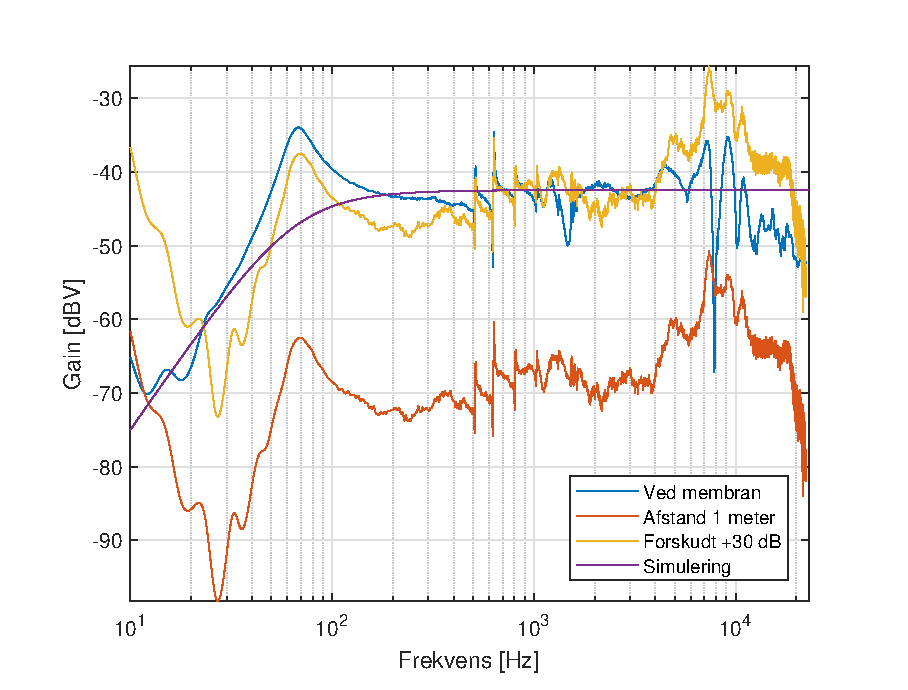
\includegraphics[width=\textwidth]{Billeder/Grafer/ClosedCabinet}
	\caption{Målinger på et lukket kabinet}
\end{figure}

Disse måleresultater udtaler sig som sagt ikke om hvordan basrefleksen påvirker frekvenskarakteristikken - men de vil blive brugt som referencemålinger i mange af de følgende måleopstillinger og resultater.\fxnote{bør vi tilpasse trykket den anden vej, så den kan sammenlignes med de psyko-akustiske kurver? - AB}

\begin{wrapfigure}{r}{0.5\textwidth} 
	\vspace{-20pt}
	\begin{center}
		\includegraphics[width=0.5\textwidth]{Billeder/FrekvenskarakteristikTeori}
	\end{center}
	\vspace{-15pt}
	\caption{Teoretisk frekvenskarakteristik}
	\vspace{-20pt}
\end{wrapfigure}
På figuren ovenfor optræder nogenlunde den type karakteristik vi forventer. Det er især resonansfrekvensen $f_s$ ved \SI{70}{\hertz} som er meget interessant idet denne frekvens adskiller det \textbf{fjederstyrede område} fra det \textbf{massestyrede område}. Derudover er der blevet målt en hældning på kurven svarende til omkring +18 dB/oktav i det fjederstyrede område - altså en smule mere end den teoretiske stigning på 12 dB/oktav.

\newpage
For at kunne sammenholde de målte data med de simulerede data, så er der blevet tilføjet en simuleret kurve på grafen ovenfor. Kurvens placering på Y-aksen er dog arbitrær og vil kun afhænge af forstærkningen i højtaleren. Den simulerede kurve har dog ingen peak ved sin resonansfrekvens - \fxnote{hvorfor har den ikke det? - TS} men den tilsvarende frekvens vil være \SI{-3}{\decibel}-frekvensen som ligger ved \SI{86}{\hertz}; altså \SI{16}{\hertz} over den målte.

På grafen ses det også, at når CLIO-mikrofonen flyttes længere væk fra membranen, så bevarer karakteristikken nogenlunde sin form omkring resonansfrekvensen - men bliver blot dæmpet med omkring \SI{30}{\decibel}. Denne dæmpning er forsøgt vist på grafen (gul)

Ved de laveste frekvenser (under \SI{20}{\hertz}) ligner to former ikke længere hinanden. Dette er dog under det hørbare spektrum og er ikke interessant for disse målinger, men den kan skyldes, at dæmpningsfaktoren i luft er meget anderledes ved lave frekvenser i forhold til høje frekvenser.

På samme måde begynder to grafer at afvige fra hinanden ved frekvenser over \SI{1000}{\hertz}. Dette passer dog fint med, at højtaleren bevæger sig ind i et frekvensområde, hvor karakteristikken i større og større grad bliver afhængig af direktiviteten. Det er altså meget muligt, at CLIO-mikrofonen ikke blev placeret præcist lige ud for højtalermembranen.

For at eftervise at de fundne målinger, så ses der på den nedenstående formel; som giver en sammenhæng mellem lydtryk og afstand fra lydgiveren:
\begin{equation}
L_2 = L_1 - \left| 20 \cdot \log \left( \frac{r_1}{r_2} \right) \right|
\end{equation}

Hvor værdierne $L_1$ og $L_2$ er lydtryksniveauet målt i afstandene $r_1$ og $r_2$. Hvis der ses peaken omkring den første resonansfrekvens $f_s$, så ligger denne ved omkring $-\SI{34}{\decibel}$ når der måles tæt på højtaleren og $-\SI{62.5}{\decibel}$,\fxnote{samme her. Skal vi hæve trykket den anden vej? - AB} når der måles i 1 meters afstand. Hvis disse værdier indsættes i den førnævnte formel, så findes der følgende:
\begin{equation}
\SI{-62.5}{\decibel} = \SI{-34}{\decibel} - \left| 20 \cdot \log \left( \frac{r_1}{\SI{1.00}{\meter}} \right)\right| \quad \Rightarrow \quad r_1 \approxeq \SI{3}{\centi\meter}
\end{equation}

Hvilket altså vil sige, at CLIO-mikrofonen har været placeret omkring \SI{3}{\centi\meter} fra højtaleren. Dette virker også meget sandsynligt.
\newpage
\subsection{Indflydelse af basrefleksens længde}
I dette afsnit vil der blive set på, hvordan længden af basrefleksen kommer til, at spille en rolle i kabinettets samlede frekvenskarakteristik. For at holde variabel-kontrol, så bliver der i første omgang kun målt på betydningen af længden, når basrefleksen er placeret på forsiden af kabinettet.

Der ønskes målt på to dele af højtalerkabinettet: Membranen og basrefleksrøret. Dette gøres ved, at placere CLIO-mikrofonen helt op ad membranen eller helt inde i basrefleksrøret. De to målinger kommer måske ikke til, at være helt akustiske adskilte, men dette er en fejlkilde man er nødt til at leve med.

I første omgang måles der kun på selve membranen, når basrefleksen sidder på forsiden. Resultaterne af disse målinger bliver opvejet med de målinger som blev fundet når kabinettet var helt lukket (ingen basrefleks). Resultatet af dette ses nedenfor.
\begin{figure}[H]
	\centering
	\vspace{-12pt}
	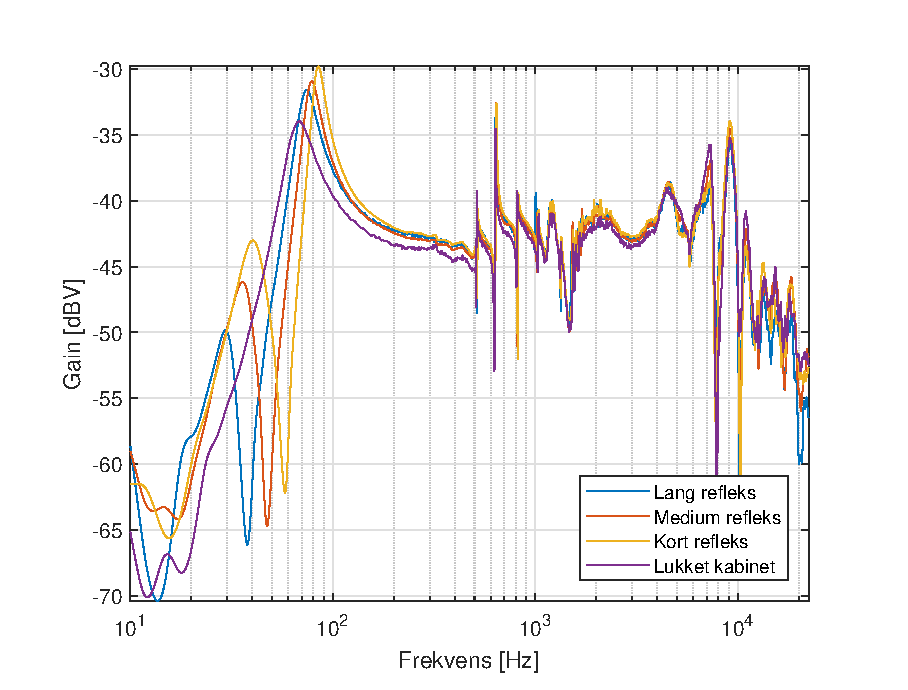
\includegraphics[width=\textwidth]{Billeder/Grafer/BasrefleksLengthMembran}
	\caption{Betydning af basrefleksens længde (målt på membran)}
\end{figure}

Det centrale ved de ovenstående måleresultater er, at der nu forekommer et 'forstærkningsdyk' omkring de lave frekvenser. Samtidig ændres både resonansfrekvensen $f_s$ placering og forstærkningen ved resonansfrekvensen, når der tilføjes en basrefleks eller ændres på længden af basrefleksen.

Det ses på figuren, at jo kortere basrefleksen bliver, jo højere op i både frekvens og forstærkning kommer resonansfrekvensen $f_s$. Samtidig ses det også, at jo længere basrefleksen bliver, jo længere ned i frekvens kommer forstærkningsdykket til at ligge, men at forstærkningen under denne faktisk stiger.

Næste skridt er, at se på selve basrefleksrørets frekvensrespons
\begin{figure}[H]
	\centering
	\vspace{-12pt}
	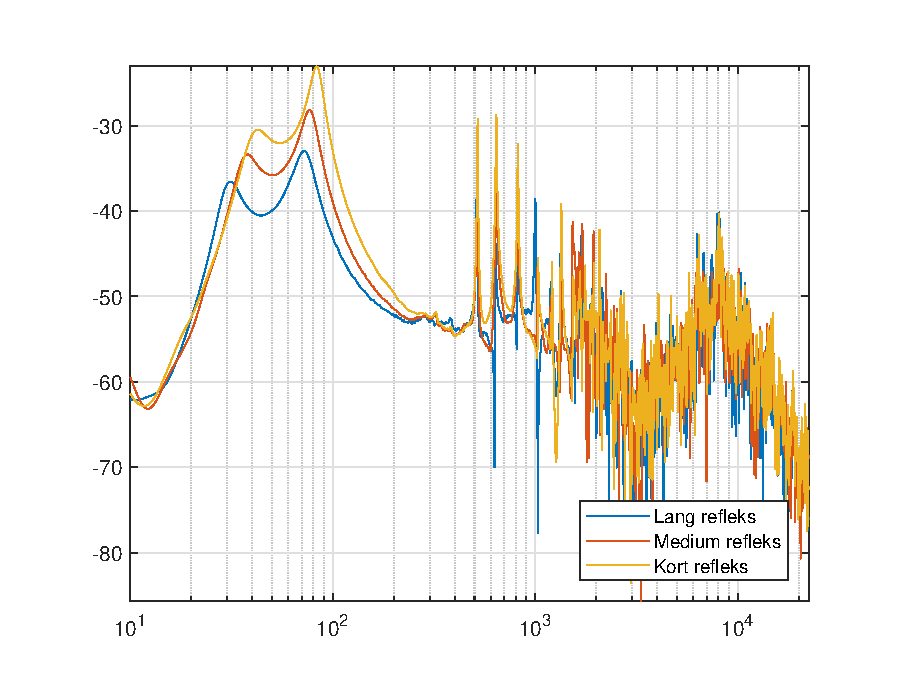
\includegraphics[width=\textwidth]{Billeder/Grafer/BasrefleksLengthTube}
	\caption{Betydning af basrefleksens længde (målt i basrefleks)}
\end{figure}
\subsection{Indflydelse af basrefleksens placering}